\documentclass[12pt]{article}

\usepackage{graphicx}
\usepackage{listings}
\usepackage{hyperref}
\usepackage{float}
\usepackage{enumitem}

\graphicspath{ {./images/} }

\oddsidemargin 0mm
\evensidemargin 0mm
\textwidth 160mm
\textheight 200mm

\pagestyle {plain}
\pagenumbering{arabic}

\newcounter{stepnum}

\title{CS/SE 2XC3 Lab 7 Report}
\author{
  Glotov, Oleg\\ L03, 400174037\\
  \texttt{glotovo@mcmaster.ca}
  \and
  Willson, Emma\\ L02, 400309856\\
  \texttt{willsone@mcmaster.ca}
  }
\date{\today}

\begin{document}

\maketitle

This report includes the main observations that we found in this week's lab, along with the analysis of our results.

\newpage 
\section{Basic Graph Algorithms}
In this section, we discuss basic graph operations and their implementations. 
\subsection{Generating Random Graphs}
We defined a function \verb+create_random_graph(n,c)+ to randomly construct a graph when given some number of nodes $n$ and number of edges $c$. The argument $c$ is given the upper bound $\frac{n\times(n-1)}{2}$ because there can be at most $\frac{n\times(n-1)}{2}$ unique edges in a graph with $n$ nodes. The algorithm initializes a graph with $n$ nodes and then generates a candidate edge between two randomly selected nodes. The candidate edge is accepted only if it is between two unique nodes (does not accept self-loops) and only if it (or its reverse) does not already exist in the graph. If a candidate edge is invalid, it is discarded and the algorithm randomly generates another one. The algorithm adds $c$ valid edges to the graph and returns the populated graph.
\subsection{Cycles Probability}
Our \verb+has_cycle(G)+ function checks if a given graph $G$ contains one or more cycles using a variation on our DFS3 algorithm. The algorithm checks for a cycle beginning at each node in the graph until it encounters one. The algorithm traverses the graph depth-first, marking visited nodes. When visiting a node, the current node and its parent are popped from the stack and the algorithm moves on to each node adjacent to the current node. If an adjacent node is unvisited, it is marked and the current and adjacent node are pushed onto the stack. If an adjacent node has been visited but is not the current node's parent, then there is a cycle and the algorithm returns true.
The minimum number of edges required for a graph to have a cycle is $3$. This is obvious because the smallest cycle possible in an undirected graph is made up of three edges. A graph with $c > k-1$ edges, where $k$ is the number of nodes, is guaranteed to have a cycle because $k-1$ is the minimum number of edges required for a connected graph. If we have a minimally connected graph with no cycles, then the addition of any edge will create a cycle. Therefore, we can expect the probability of a cycle in the 100-graph to vary between edge numbers $c=3$ to $c=99$.
\begin{figure}[H]
\centering
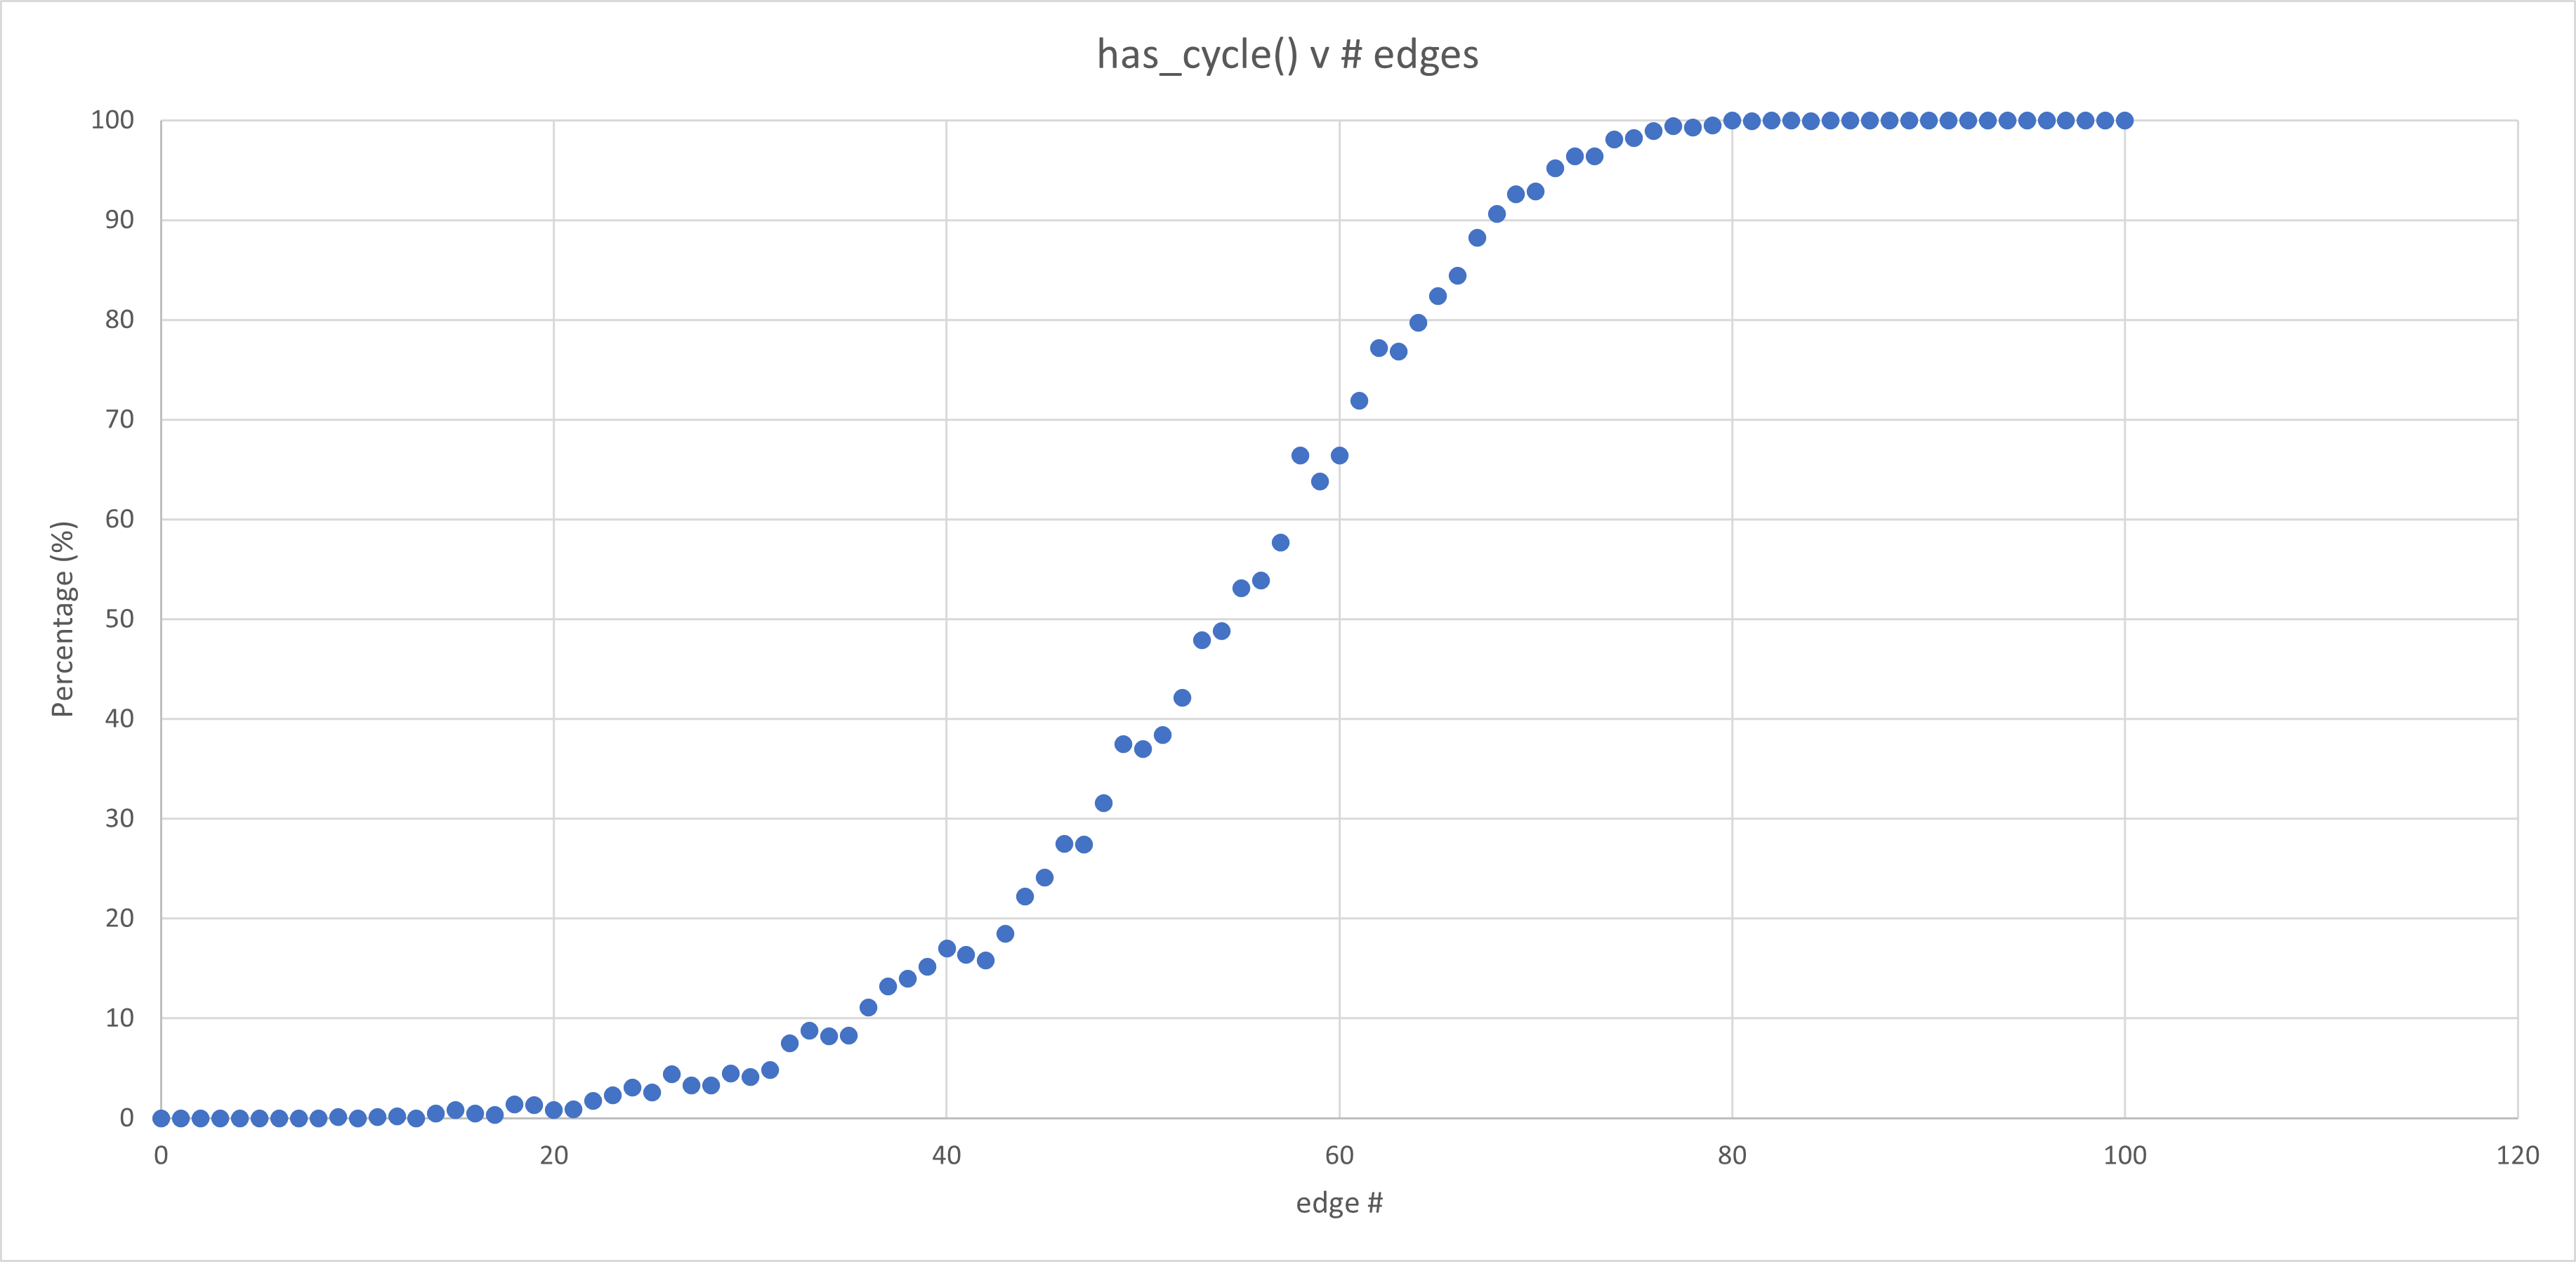
\includegraphics[width=0.9\textwidth,height=\textheight,keepaspectratio]{cycle}
\caption{probability of cycle in 100-node graph}
\label{Figure: m1}
\end{figure}
\noindent As shown in the graph above, the probability of a cycle occurring in a randomly-generated graph is at approximately 50\% when $c=54$. This is expected because 54 is almost halfway between 3 and 99. 
\subsection{Connected Probability}
Our \verb+is_connected(G)+ function checks if each node in a given graph $G$ is reachable by every other node. The algorithm performs a depth-first search using our \verb+DFS3+ function and compares the number of parent-child relations recorded in the returned parent dictionary to the number of nodes in the graph. A depth-first search on a connected graph should visit every node in the graph, so if the input graph is connected, the parent dictionary will contain a record of every node in the graph. If the number of parent records is equal to the number of nodes, the algorithm returns True. 
As stated earlier, a graph requires at least $k-1$ edges to be connected. The maximum number of unique edges a connected graph can have is $\frac{n\times(n-1)}{2}$. Therefore, we can expect the connected probability of the 100-graph to vary between edge numbers $c=99$ to $c=4950$.
\begin{figure}[H]
\centering
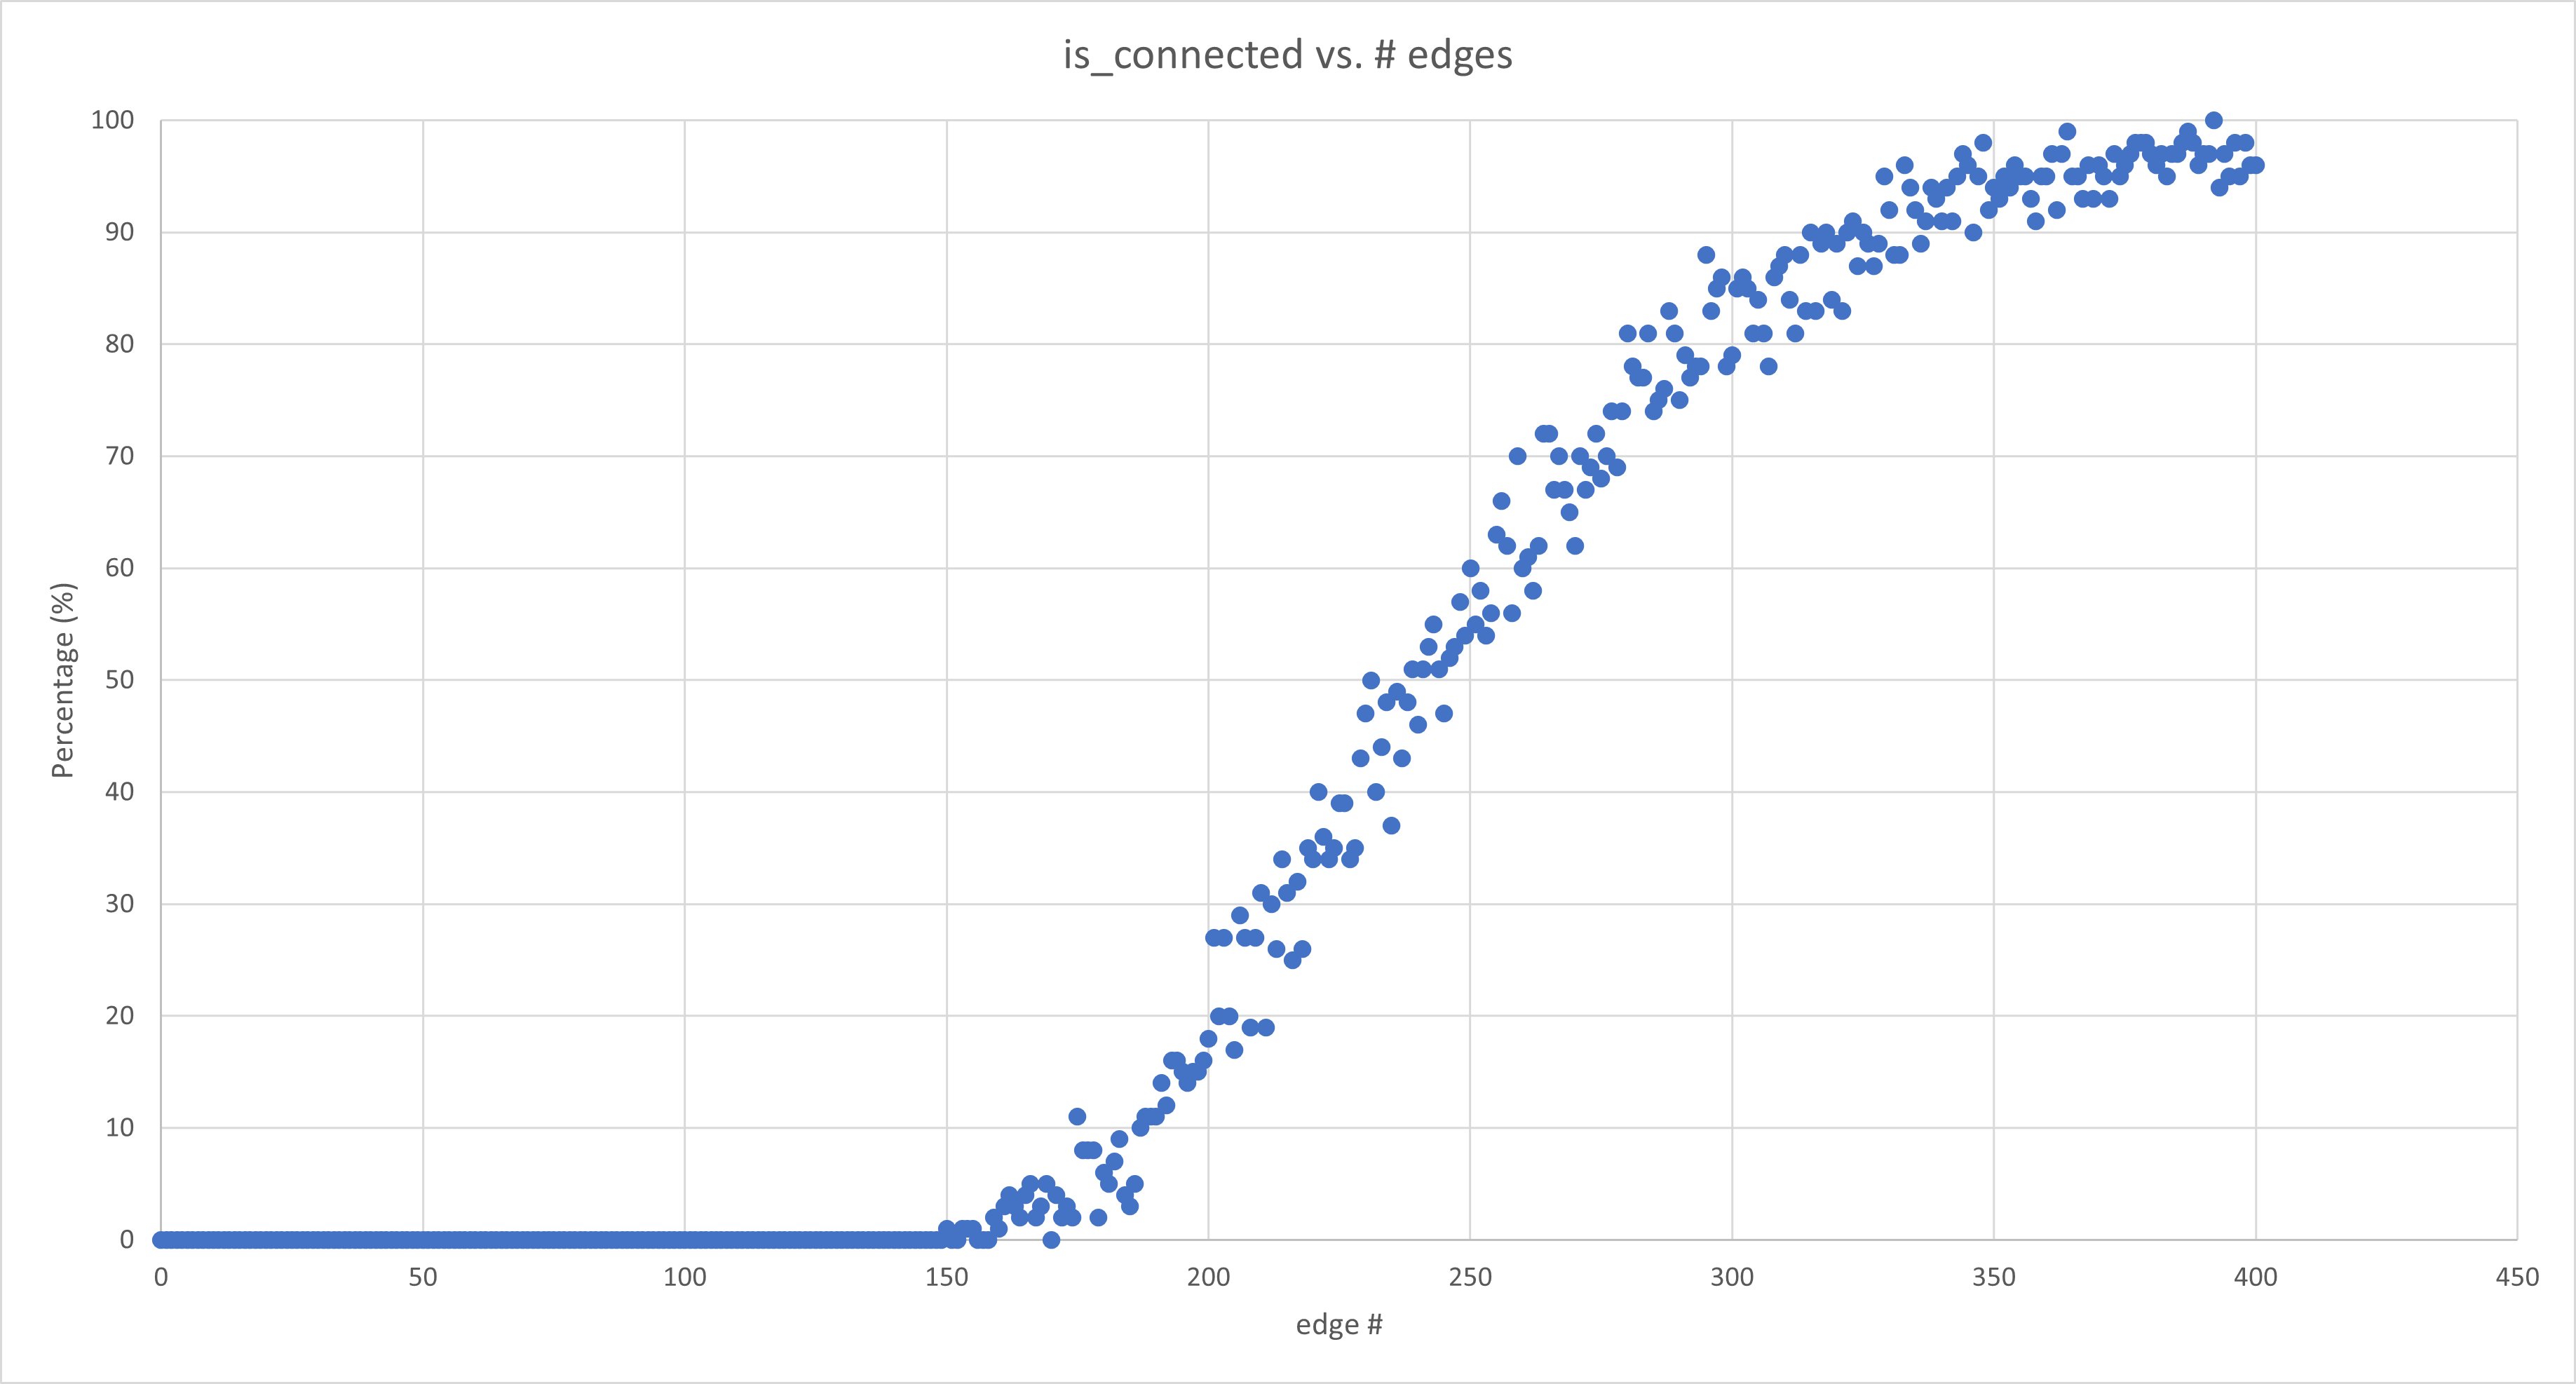
\includegraphics[width=0.9\textwidth,height=\textheight,keepaspectratio]{connected}
\caption{probability of being connected in 100-node graph}
\label{Figure: m2}
\end{figure}
As shown in the graph above, the probability of connectedness in a randomly-generated graph is at approximately 50\% when $c=244$. This is expected because 244 is between 99 and 4950. 
\subsection{Comparing c Values}
As detailed in the "is connected" section, the high "c" value is explained by the high minimum edge requirement and the low probability that all the edges will be connected. In other words, the "has cycle" has a lower requirement to return true than the "is connected" function. Therefore it makes sense the "is connected" requires a higher value for c for the graphs to be connected half the time compared to having a cycle half the time.

\end{document}

